
\chapter{Evaluierung von Net2Net}\label{sec:net2netexperimente}
Die Operatoren zur Beschleunigung des Lernens durch Wissenstransfer werden in diesem Unterkapiel evaluiert. Diese Evaluierung arbeitet mit einer selbst erstellten Implementierung auf Grundlage der Veröffentlichung zum Thema Net2Net \cite{net2net}.

Die Evaluierung umfasst drei unterschiedliche Situationen, diese Situation sind analog zu den in der dazugehörigen Quelle \cite{net2net}. Die Evaluierung arbeitet mit einem ResNet, wie in Kapitel \ref{sec:baseline}.

In der ersten Situation wird der Operator für ein breiteres Netz verwendet, um ein schmalleres ResNet32 zu trainieren. 
In der zweiten Situation wird der Operator für ein tieferes Netz benutzt um zusätzliche Blöcke hinzuzufügen oder bestehenden Blöcken Schichten hinzuzufügen. In der dritten Situation werden beide Operatoren kombiniert. Mit der Kombination wird der Raum erkundet, ausgehend von einem Modell.
Die drei Situationen werden in den drei folgenden Unterkapiteln näher beschrieben. Anpassungen der Lernrate werden erst in der dritten Situation vorgenommen

\section{Evaluierung des Operators für ein breiteres Netz}
Evaluiert wird der Operator durch verschiedene Optionen, welcher Bereich des Netzes breiter gemacht wird:
\begin{itemize}
 \item Alle Phasen
 \item Eine ganze Phase
\end{itemize}
Wie in Kapitel \ref{sec:net2net} beschrieben werden beim Operator für ein breiteres Netz die Gewichte für die neu hinzugefügten Gewichte aus den ursprünglichen Gewichten ausgewählt und so normalisiert, dass die approximierte Funktion nicht signifikant von der approximierten Funktion mit den neuen Gewichten abweicht. Um zu evaluieren wie gut diese Methode funktioniert wird sie auf das schmalle Baseline-Netz angewendet und verglichen mit dem schmallen und breiten Baseline-Netz. Um die Methode der Initialisierung der zusätzlichen Kanäle zu evaluieren wird als Vergleich ein Netz trainiert, bei welchem die zusätzlichen Gewichte zufällig initialisiert werden.
\color{blue1}

In Abbildung \ref{abb:deeper1} ist der Verlauf der Trainingsaccuracy des schmallen Baseline Netzes über 180 Epochen ohne Anpassung der Lernrate zu sehen. 



Dabei ist zu sehen, dass das Netz nicht konvergiert. Zunächst wird der Zeitpunkt gesucht, ab dem das Netz nicht mehr besser wird im Durchschnitt. Damit die Entscheidung in einer Epoche stärker von den näher liegenden vergangenen Epochen abhängig ist, wird ein exponentiell gewichteter Mittelwert berechnet. In die Berchnung eingehen werden letzten $n$ Werte, für ein festes $n$.
Abbildung \ref{abb:deeper2} zeigt den Verlauf dieses Mittelwert für $n=10$ (Blau) und $n=30$ (Grün).
\begin{figure}
     \centering
     \subfloat[][]{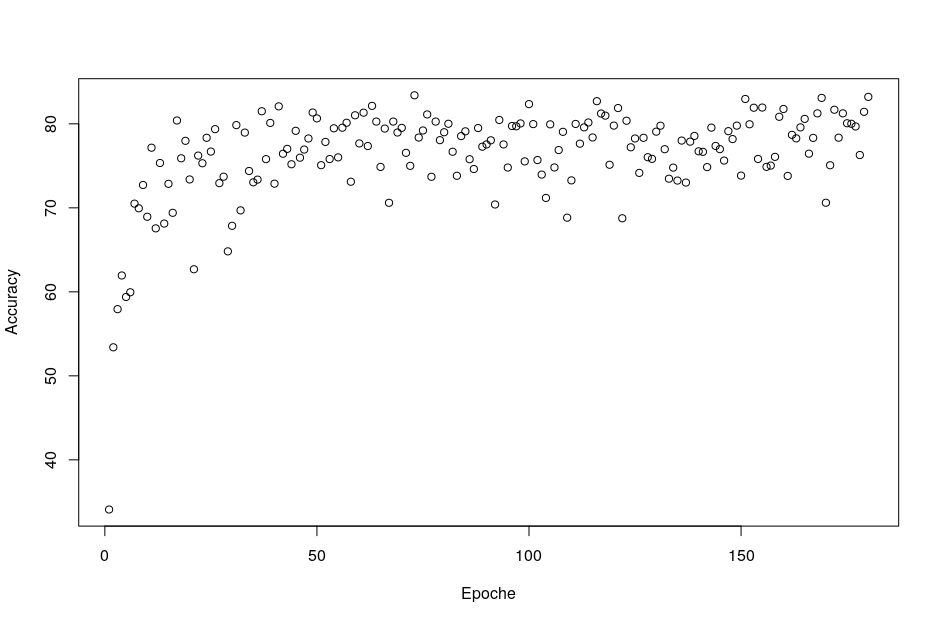
\includegraphics[width= .47\textwidth]{KapitelPartB/Images/deeperD1.png}\label{abb:deeper2}}
     \hfill
     \subfloat[][]{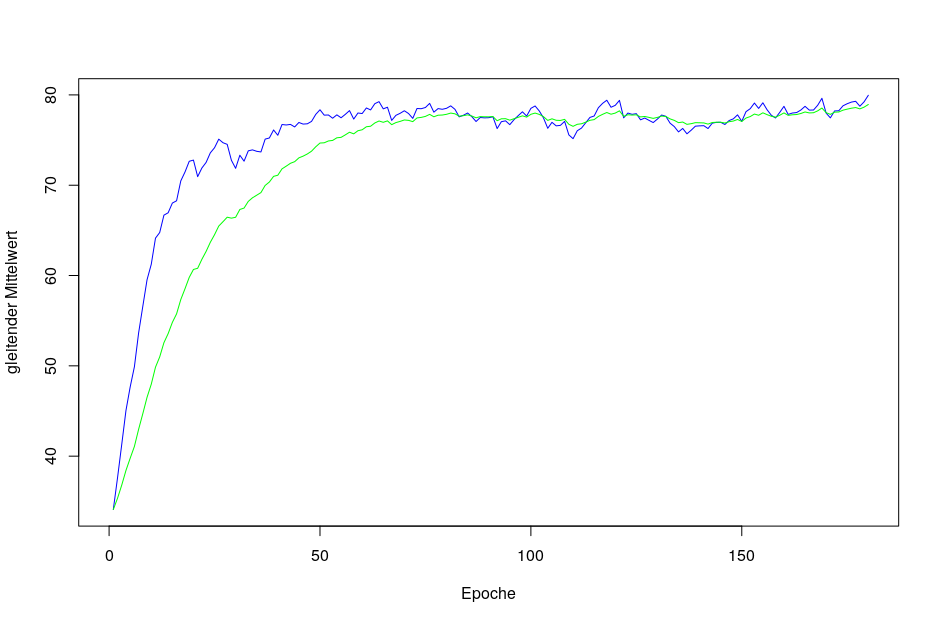
\includegraphics[width= .47\textwidth]{KapitelPartB/Images/deeperD2.png}\label{abb:deeper2}}\\
     \caption{}
     \label{abb:memory}
\end{figure}
Im nächsten Schritt muss anhand eines Entscheidungskriteriums 


\color{black}
\subsection{Verbreitern aller Phasen}
Mit Hilfe verschiedener Trainingsprotokolle wird untersucht, wie der Operator für ein breiteres Netz die Klassifikationsleistung des Netzes verändert.
Zunächst wird überprüft, welches Ergebnis bei Anwendung des Operators für ein breiteres Netz auf das schmalle Baseline-Netz nach 180 Epochen Training herauskommt. Nachdem Anwenden des Operators wird mit dem gleichen Trainingsprotokoll für weitere 180 Epochen trainiert. In Abbildung \ref{abb:allN2N1} ist abgebildet, wie der Verlauf der Accuracy für Net2Net mit zwei verschiedenen Möglichkeiten, die neuen Gewichte zu initialisieren, ist. In Blau dargstellt wird der Verlauf der Accuracy für die zufällige Initialisierung der neuen Gewichte durch das Verbreitern des Netzes.
Es ergibt sich, wie in der größeren Abbildung \ref{abb:allN2N2} zu sehen ist eine minimale Verschlechterung durch das Anwenden des Operator für ein breiteres Netz im Vergleich zum Baseline-Netz.
 \begin{figure}
     \centering
     \subfloat[][]{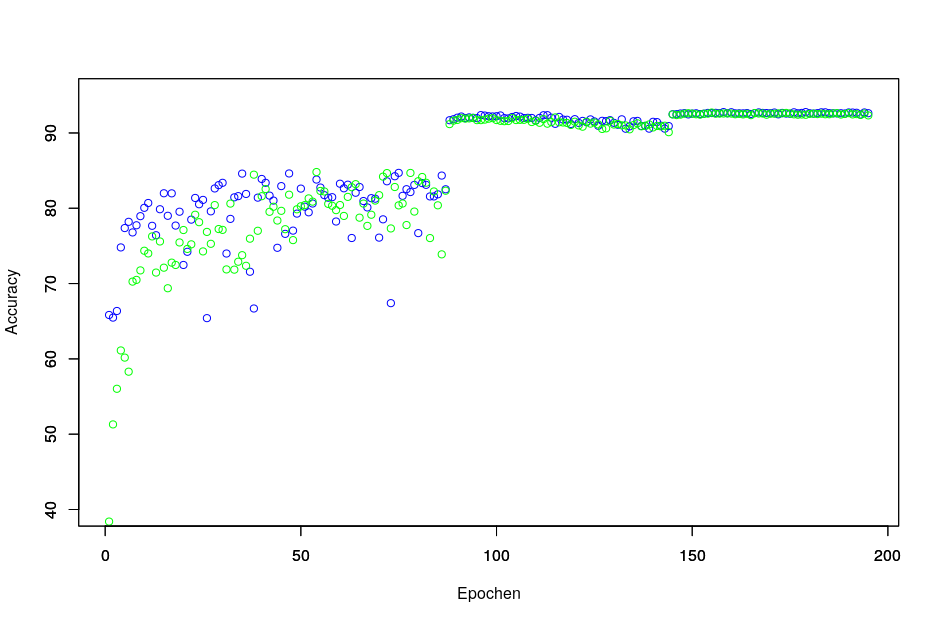
\includegraphics[width= .47\textwidth]{KapitelPartB/Images/n2nWiderAll1.png}\label{abb:allN2N1}}
     \hfill
     \subfloat[][]{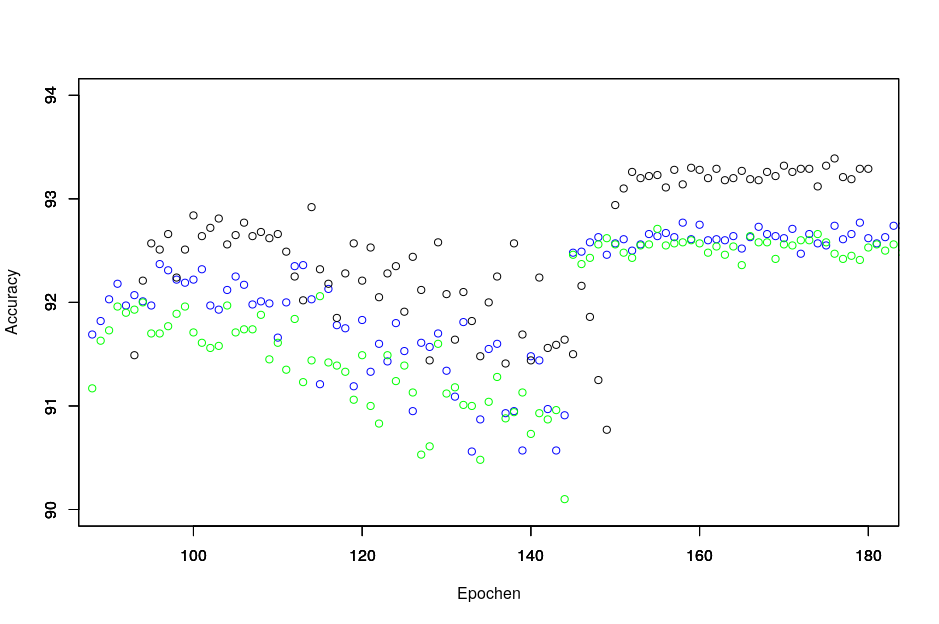
\includegraphics[width= .47\textwidth]{KapitelPartB/Images/n2nWiderAll2.png}\label{abb:allN2N2}}\\
     \caption{Vergleich der Accuracy bei verschiedenen Initialisierungsmöglichkeiten des Operators für ein breiteres mit dem Baseline Netz: (a) alle Epochen (b) Zoom auf die Epochen 90 bis 180. Blau zeigt die Accuracy der Initialisierung der zusätzlichen Gewichte mit zufälligen Werten. Grün zeigt die Initialisierung mit den Werten aus dem restlichen Tensor. Schwarz zeigt das Baseline-Netz als Vergleich.}
     \label{abb:memory}
\end{figure}
Um den Operator für ein breiteres Netz besser verwenden zu können wird im nächsten Schritt übrprüft, ob mit einer häufigeren schrittweisen Anpassung der Lernrate und mit weniger trainierten Epochen nach Anwenden des Operator ein besseres Ergebnis möglich ist.


\section{Evaluierung des Operators für ein tieferes Netz}
Zur Evaluierung des breiteren Netzes wird zunächst wie in der Veröffentlichung jeder Block um eine Schicht erweitert. Dabei werden die zusätzlichen Schichten wie in Kapitel \ref{sec:deep} beschrieben initialisiert. Als Vergleich dient das Baseline-Netz aus Kapitel \ref{sec:baseline}.

\todo{Ergebnisse}

Eine weitere Verwendung des Operators für ein tieferes Netz ist die Möglichkeit einen neuen Block hinzuzufügen. Nur ein einfaches Hinzufügen würde hier zu Problemen führen. Der Grund hierfür ist Abbildung \ref{abb:deeper} dargstellt. Dabei soll an einer Verbidung, die bisher die Daten von einer Schicht zur nächsten transportiert ein neuer Block inklusive Kurzschlussverbindung entstehen. Der hinzuzfügende Block blau \todo{blau markieren} markiert. Der neue Block soll wie die Kurzschlussverbindung die Identität berechnen. Betrachtet $x$ als Größe der Identität. Dann wird hier mit dem neuen Block staat $x$ das doppelte, also $``X$ berechnet. Um dieses Problem zu umgehen wird an jeder Additionsstelle für eine Kurzschlussverbindung eine Multiplikation mit 0,5 berechnet (rechte Seite der Grafik). So wird nicht mehr $x$ sondern $0,5x +0,5x=x$ berechnet.

Zunächst wird dieses Netz trainiert ohne einen Operator anzuwenden. In Abbildung \ref{abb:BaselineMul1} ist ein Boxplot abgebildet, der die Accuracy des Netzes mit zusätzlichen multiplikativen Faktoren mit dem Baseline-Netz vergleicht.

 \begin{figure}
     \centering
     \subfloat[][]{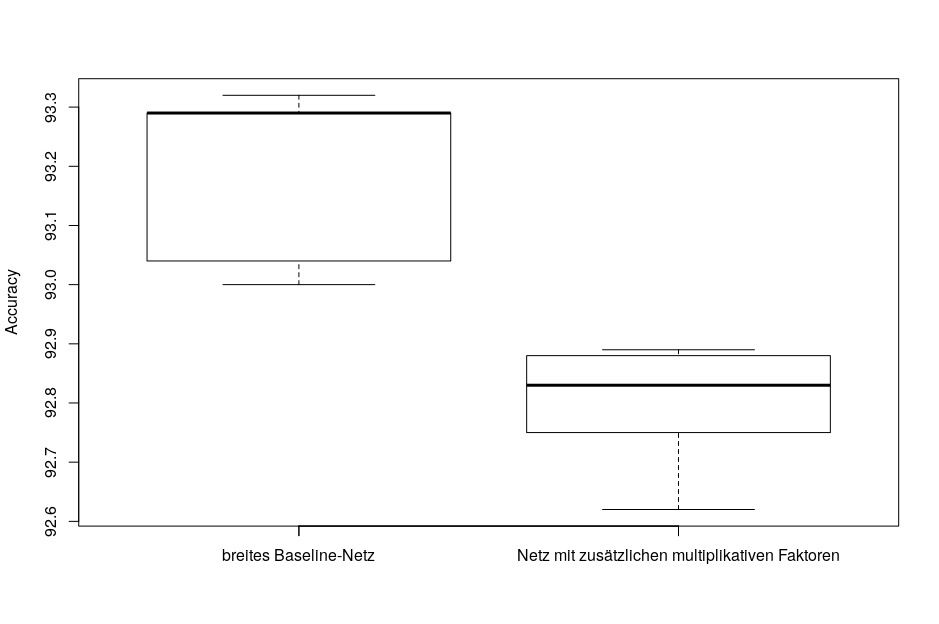
\includegraphics[width= .75\textwidth]{KapitelPartB/Images/baselineMul1.png}\label{abb:BaselineMul1}}
     \hfill
     \caption{Vergleich von }
     \label{abb:BaselineMul}
\end{figure}


\begin{figure}[h]
 \centering
 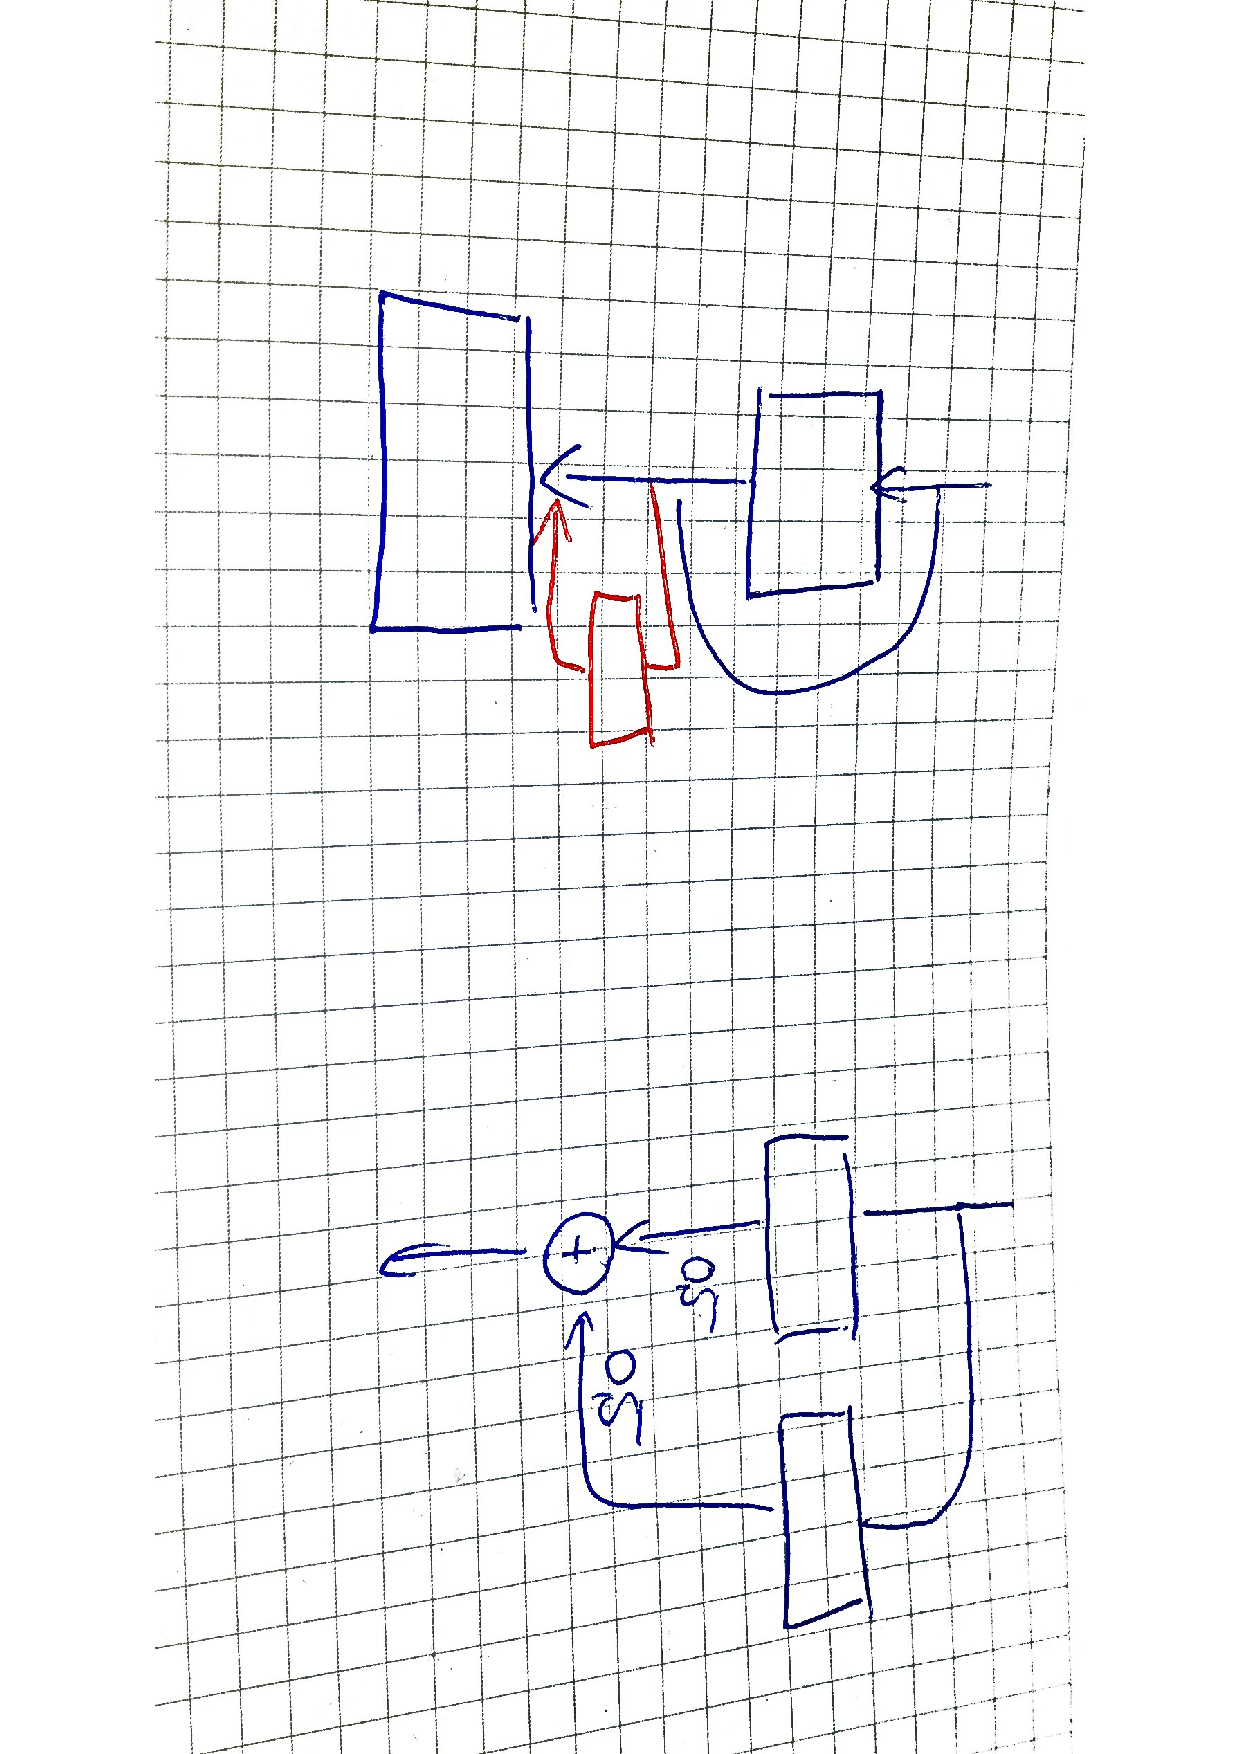
\includegraphics[width=0.5\textwidth, angle=90]{KapitelPartB/Images/deeper.pdf}
 % deeper.pdf: 0x0 px, 300dpi, 0.00x0.00 cm, bb=
 \label{abb:deeper}
\end{figure}




\section{Erkunden des Modellraums}

 \begin{figure}
     \centering
     \subfloat[][]{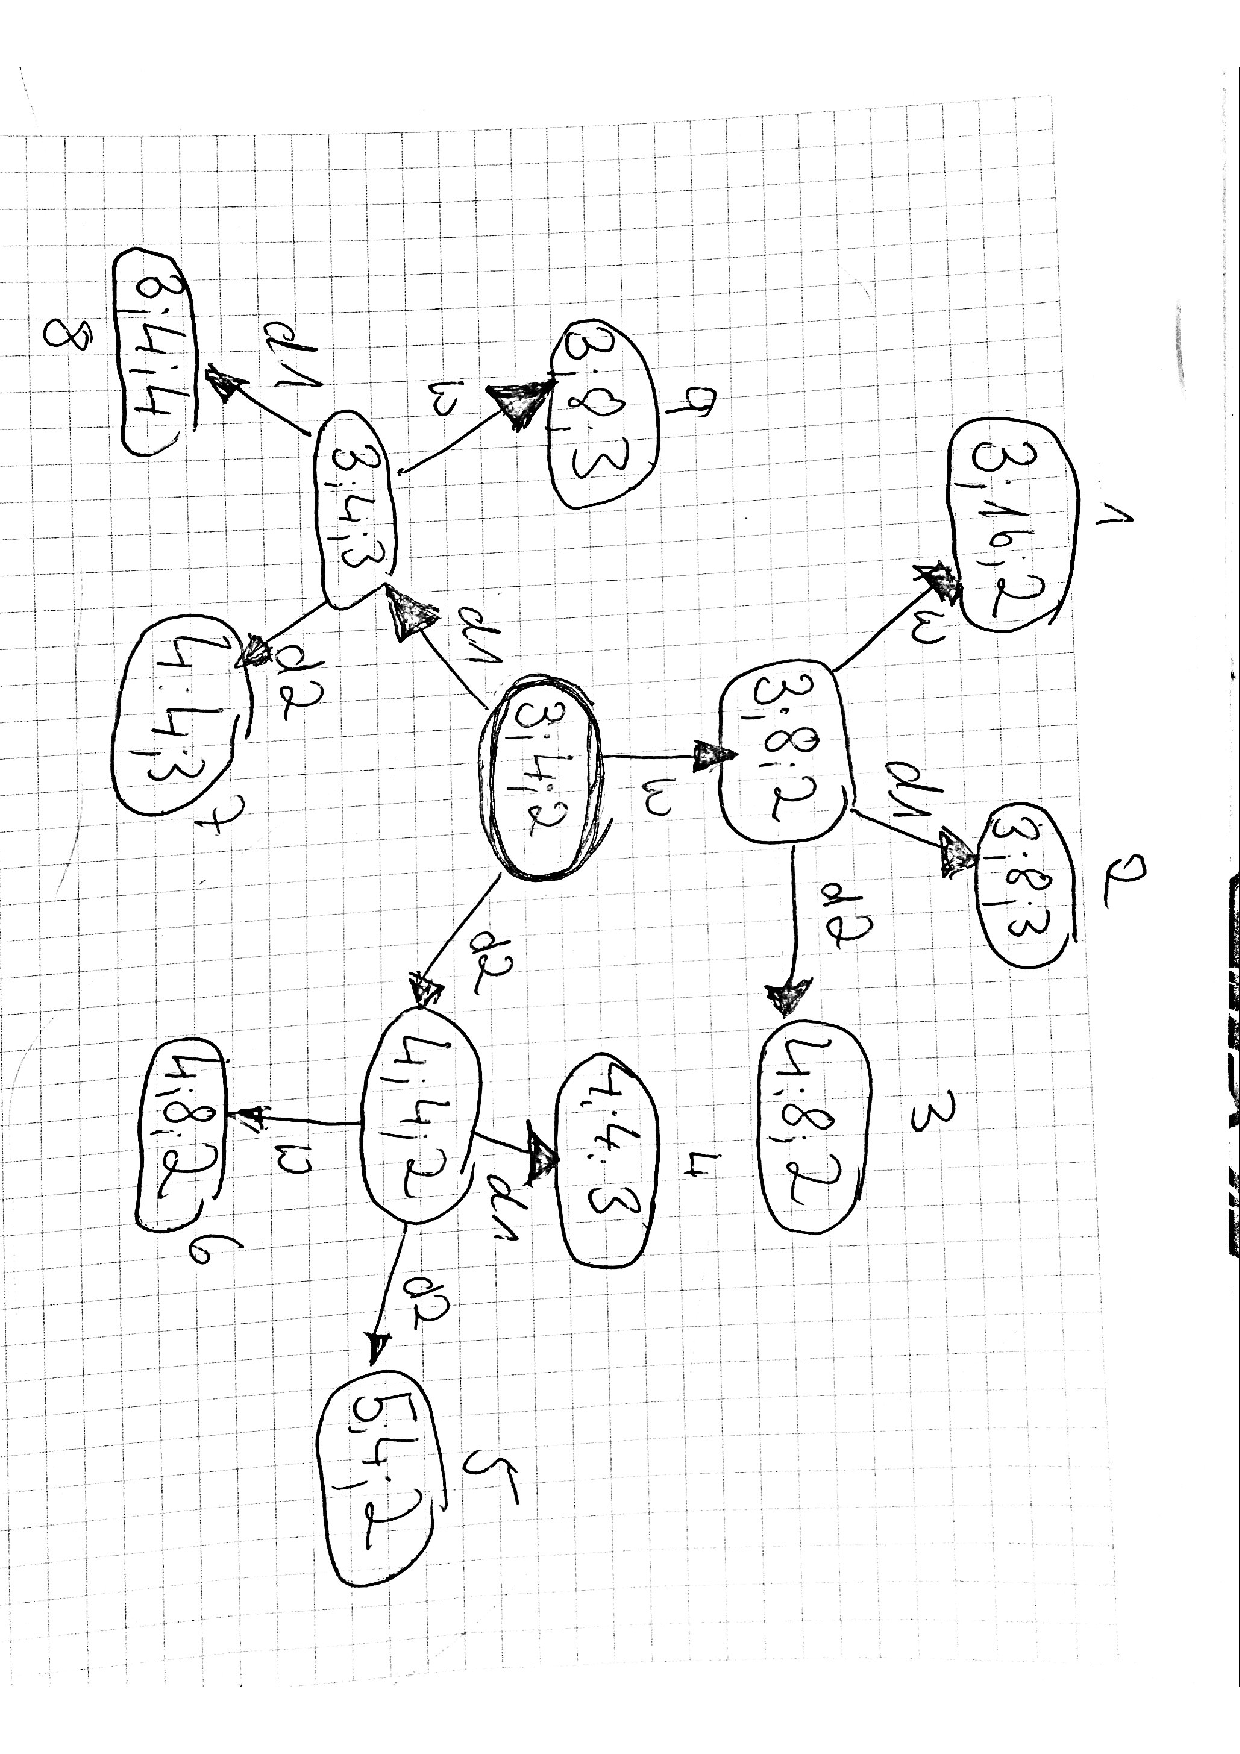
\includegraphics[width= .75\textwidth, angle=90]{KapitelPartB/Images/deeperRoom.pdf}
     \label{abb:deeperRoom1}}
     \caption{Anzahl an Blöcken pro Phase; Breite der ersten Schicht; Schichten pro Block}
     \hfill
\end{figure}

